\documentclass[letterpaper]{article}
\usepackage{alifeconf}
\usepackage[utf8]{inputenc}
\usepackage{hyperref,mathtools}
\graphicspath{{images/}}

\title{A ship routing algorithm and it's map visualization}
\author{Andreas Lorer \and  Kevin Klugmann\\
\mbox{}\\
Hochschule Ravensburg-Weingarten, Doggenriedstr. 88250 Weingarten \\
contact@andreaslorer.de, kevin.klugmann@gmail.com}


\begin{document}
\maketitle

\begin{abstract}
Lorem ipsum dolor sit amet, consectetur adipisicing elit, sed do eiusmod
tempor incididunt ut labore et dolore magna aliqua. Ut enim ad minim veniam,
quis nostrud exercitation ullamco laboris nisi ut aliquip ex ea commodo
consequat. Duis aute irure dolor in reprehenderit in voluptate velit esse
cillum dolore eu fugiat nulla pariatur. Excepteur sint occaecat cupidatat non
proident, sunt in culpa qui officia deserunt mollit anim id est laborum.
\end{abstract}

\section{Introduction}
	Während es beim Nahverkehr sehr einfach ist, eine Route zu berechnen\footnotemark und in einer interaktiven Karte zu visualisieren, so gibt es zum jetzigen Zeitpunkt keine Möglichkeit dies für Schiffsrouten zu tun. Abbildung \ref{fig:visualisierungsproblem} zeigt eine Visualisierung wie sie momentan in einer Karte zum Einsatz kommt. 

	\footnotetext{Via Google-Maps, Bing-Maps oder weiteren Kartenanbieter}

	\begin{figure}[!htb]
		\begin{center}
		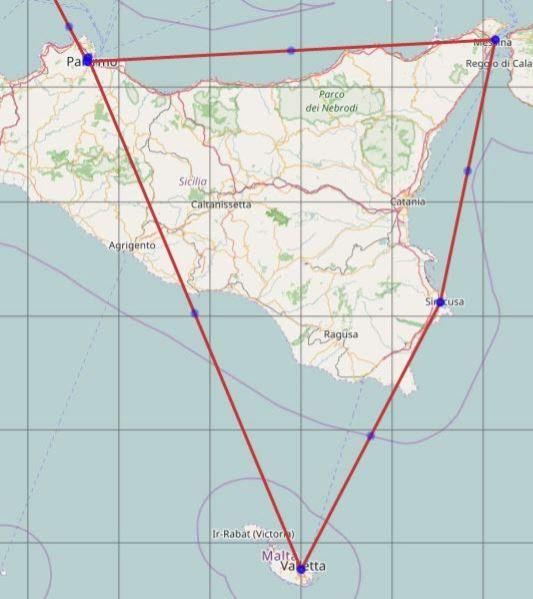
\includegraphics[width=2in]{visualisierungsproblem}
		\caption{Beispiel einer Kartenvisualisierung}
		\label{fig:visualisierungsproblem}
		\end{center}
	\end{figure}

	Die Grafik veranschaulicht auch gleichzeitig das Problem: Die einzelnen Häfen sind nur durch gerade Linien verbunden, die nicht zwischen Wasser und Land unterscheiden. Dadurch führen Routen über Land. Für dieses Problem der automatischen Kartengenerierung wurde ein Algorithmus entwickelt. Dieser ist in der Lage Land und Wasser zu unterscheiden und damit ein visuell ansprechendere Visualisierung zu ermöglichen. Als Eingabe nimmt der Algorithmus eine Liste an Hafen-Positionen und generiert daraus eine Route. Eingabe und Ausgabe werden dabei im \texttt{geojson-Format} \cite{rfc7946} eingelesen beziehungsweise ausgegeben.

	Momentan werden Routen für die Kreuzschifffahrt vorwiegend auf zwei Arten visualisiert.

	\begin{figure}[!htb]
		\begin{center}
		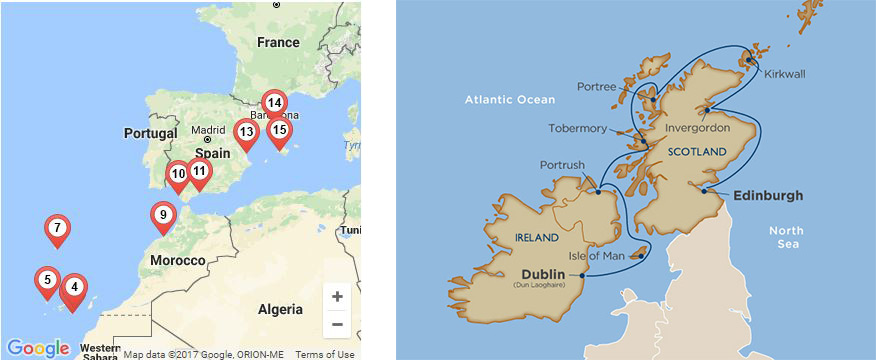
\includegraphics[width=\linewidth]{state_of_the_art}
		\caption{State of the art}
		\label{fig:state of the art}
		\end{center}
	\end{figure}

	Wie in Abbildung \ref{fig:state of the art} zu sehen ist, werden entweder nur einzelne Pin's auf die jeweiligen Häfen gesetzt oder es werden aufwendige Vektorgrafiken händisch erzeugt. Letzteres ist dabei sehr aufwändig und dadurch teuer. Einzig \url{http://www.cleancruising.com.au/} hatte eine visuell überzeugende Karte (Abbildung \ref{fig:state of the art cleancruise}) mit einem ansprechendem Routing. 

	\begin{figure}[!htb]
		\begin{center}
		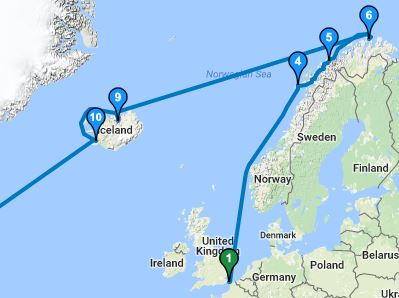
\includegraphics[width=.6\linewidth]{state_of_the_art_cleancruise}
		\caption{Kartenvisualisierung von cleancruise.com}
		\label{fig:state of the art cleancruise}
		\end{center}
	\end{figure}

	Für unseren Algorithmus geht es dabei nicht unbedingt um die Routenberechnung im klassischen Sinne (kürzester Weg), sondern um eine ästhetische Darstellung. Die Zielgruppe sind Personen die mittels eines Buchungsportals eine Kreuzfahrt buchen wollen. Die Route hat also keinerlei Relevanz für Nautiker oder Kapitäne. Wassertiefe oder nicht befahrbare Abschnitte sind für uns nicht zu beachten. 

	Andere Bedingungen für einen Algorithmus sind oftmals seine lineare Laufzeit $O(n)$ die für Echtzeitsysteme benötigt werden. Unser Algorithmus ist allerdings nur für den Einsatz im Backend vorhergesehen. Dort werden die Routen für die Anzeige im Frontend bereits vorberechnet und zur wiederverwendung abgespeichert. Eine lineare Laufzeit ist dadurch nicht von nöten und war zu keiner Zeit eine Anforderung.

\section{Related Work}
	Es gibt nicht viel an Publikationen, die sich mit dem Thema Schiffsrouten via Web-Plattform auseinandersetzen.\\

	Die meisten Systeme die Routenberechnungen für die Schiffahrt durchführen, benutzen eine Graph basierte Grid-Struktur oder eine Abwandlung davon. \cite{makrygiorgos15} entwickelte Beispielsweise eine \texttt{Novel Grid Structur} (siehe Abbildung \ref{fig:novel grid structure}). In dieser Datenstruktur wird für jeden Knotenpunkt (Node) maritime Informationen abgespeichert und gewichtungen für jede Kante (Edge) berechnet.

	\begin{figure}[!htbp]
		\centering
		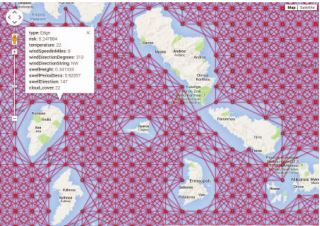
\includegraphics[width=.8\linewidth]{novel_grid_structure}
		\caption{Novel Grid Structure (Abbildung von \cite{makrygiorgos15})}
		\label{fig:novel grid structure}
	\end{figure}

	Die Motivation dahinter ist dabei meistens ein Echtzeitsystem oder eine Echtzeitkalkulation der Route. Eine Grid-Struktur, die wie ein Graph aufgebaut ist, beschleunigt den Suchprozess des A*-Algorithmus erheblich\cite{patel16}. Die Grid-Struktur wird dabei aus den statischen maritime Informationen und zusätzlichen dynamischen Daten (meterologische Wetterdaten über Windstärke, Windrichtung etc) für die Routenberechnung ergänzt \cite[s. 2]{makrygiorgos15}.
	Für unseren Algorithmus wäre es zwar hilfreich gewesen eine solche Datenstruktur zu haben, allerdings verfügten wir über keinerlei Zugriff auf solche Datenquellen, da diese unseren Recherche nach nicht öffentlich frei verfügbar sind.

\section{Die Pixel-Karte}
	In diesem Abschnitt erklären wir unsere Arbeit an dem Routing Algorithmus für Kreuzschiffsfahrten. Alles basiert auf der generierung einer Pixel-Karte. Diese Karte dient uns als Grundlage für das Routing mittels A*-Algorithmus. Die Pixel-Karte aus Abbildung \ref{fig:Pixel Map Miami} wird durch Kartendaten von Natural Earth\footnotemark auf einem HTML5-Canvas erzeugt. 

	\footnotetext{Natural Earth 1:10m coastline \url{http://bit.ly/2kbyYIV}}

	\begin{figure}[!htbp]
		\centering
		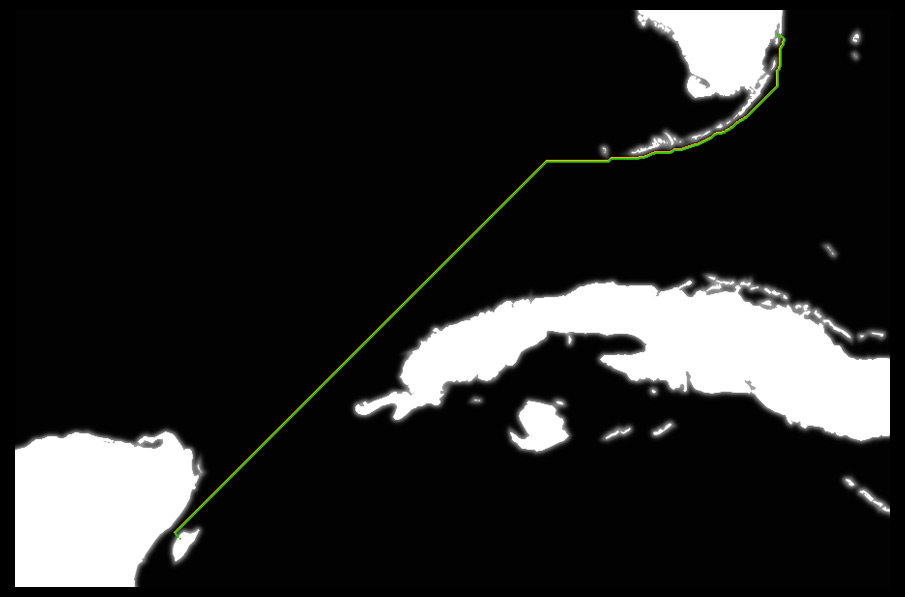
\includegraphics[width=\linewidth]{pixel_map_miami}
		\caption{Generierte Pixel-karte für eine Routenberechnung}
		\label{fig:Pixel Map Miami}
	\end{figure}

	Der Maßstab der Karte beträgt dabei 1:10m (millionen) und liegt im Datenformat \texttt{.shp} (für Shapefile) vor. Diese wurde mittels eines Tools (QGIS) in \texttt{geojson} umgewandelt. Höher aufgelöstest Kartenmaterial ist im Netz an verschiedenen Stellen zu finden\footnotemark, diese haben dann allerdings Dateigrößen von bis zu 500 MB. Da wir solch hohe Datenmengen Client-Seitig nicht verarbeiten konnten, ist für uns die Karte mit Maßstab 1:10m ein solider Kompromiss zwischen nötiger Genauigkeit entlang der Küstenlinie (Inseln \& Fjorde etc.) und Datengröße.

	\footnotetext{z.B. bei OpenStreetMap \url{http://openstreetmapdata.com/data/coast}}

	Nachdem die Pixel-Karte auf den Canvas gezeichnet ist, dient uns die Canvas-Auflösung als Grid-Raster. Höhere Auflösungen ermöglichen es dabei, mehr Details darzustellen. Das ist besonders für Fjorde und Inseln nötig, da diese bei einer zu niedrig aufgelösten Pixel-Karte nicht dargestellt werden können. Eine Auflösung von $512^2$ oder $1024^2$ wurde dabei bei unseren Routenkalukationen als ein solider Wert befunden und erzeugte gute Ergebnisse. Je höher die gewählte Auflösung, umso mehr Arbeitsspeicher wird allerdings auch benötigt. Da wir Client-Seitig eine limitierung des verfügbaren Arbeitsspeichers durch den Browser haben, konnten höhere Kartenauflösungen nicht getestet werden. Sobald eine Portierung auf eine Server-Seitige Lösung via Node.js erfolgt, sollte dies allerdings möglich sein.

	\subsection{Pixel-Karte in Graustufen}
		Der HTML5 Canvas bietet die Möglichkeit, die Farbinformationen für jeden Pixel auszulesen. Ein schwarzer Pixel bedeutet dabei, dass es sich um Wasser handelt und ein weißer Pixel folglich um Land, also ein Hindernis. Aber nur die Unterscheidung zwischen Land und Wasser würde zu dem Problem führen, dass Schiffe genau entlang der Küstenlinie fahren würden, da dies der kürzeste Weg von A nach B darstellt (siehe Abbildung \ref{fig:route before blur}).

		\begin{figure}[!htbp]
			\centering
			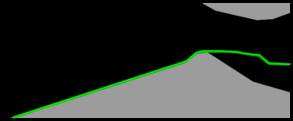
\includegraphics[width=.8\linewidth]{route_before_blur}
			\caption[]{Pixel Karte vor dem Blur-Effekt.\footnotemark}
			\label{fig:route before blur}
		\end{figure}
		\footnotetext{Das Land wurde ausgegraut, um die Route besser sichtbar zu machen}

		Schiffe fahren aber nicht genau auf der Küstenlinie, sondern nur in Küstennähe.

		Um dieses Problem zu lösen und eine glaubhaftere Schiffsroute zu generieren, musste die berechnete Route von der Küstenlinie versetzt werden. Dafür haben wir die Pixel-Karte einer Manipulation unterzogen, welche in Abbildung \ref{fig:blur effect} zu sehen ist. Dabei sind zwei Schritte nötig. Erstens wird die Pixel-Karte 3 mal gezeichnet. Dabei wird die Pinselgröße des Canvas jedes mal verringert (auf 6, 3, 0.1). Bevor dann in der letzten Iteration das Land gezeichnet wird, erfolgt noch ein Gaussian Blur Filter\cite{vigour17}. Dieser bewirkt, dass die sehr harten Kanten, die beim Zeichnen entstehen, geglättet werden und ein homogener Übergang erreicht wird.

		\begin{figure}[!htbp]
			\centering
			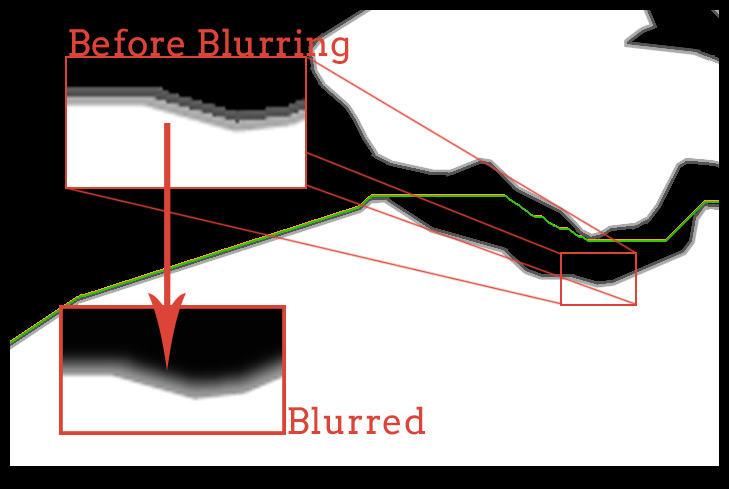
\includegraphics[width=\linewidth]{blur_effect}
			\caption{Anwendung eines Gaussian-Blur Filters}
			\label{fig:blur effect}
		\end{figure}

		Nach dem Anwenden des Blur Filters wird dann als letztes die Landmasse eingezeichnet, damit diese ihre scharfe Kante behält und nicht durch den Blur in unschärfe verschwimmt.

		\begin{figure}[!htbp]
			\centering
			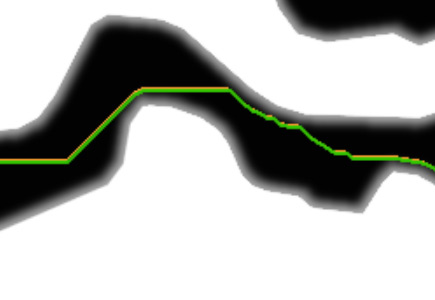
\includegraphics[width=\linewidth]{route_after_blur}
			\caption{Ergebnis der Routenberechnung mit Blur Filter Pixel-Karte}
			\label{fig:route after blur}
		\end{figure}

		Wie in Abbildung \ref{fig:route after blur} zu sehen ist, wurde die Route weg von der Küstenlinie geschoben und sieht nun visuell mehr wie eine reale Schiffahrtsroute aus, die zum Beispiel dem einem zu niedrigem Fahrwasser ausweichen würde.



{\footnotesize \bibliographystyle{acm}
\bibliography{references}}

\end{document}
